\documentclass[10pt, compress]{beamer}

\usetheme{m}

\usepackage{booktabs}
\usepackage[scale=2]{ccicons}
\usepackage{minted}
\usetikzlibrary{calc, arrows}
\usepackage{xstring}
\usepackage{amsmath}
%\usepackage[chromatogram,domains]{pgfmolbio}
\usetikzlibrary{decorations.fractals}
\usepgfplotslibrary{dateplot}

\usemintedstyle{trac}

\usepackage{tikz}
\usetikzlibrary{shapes,arrows}
\tikzstyle{cloud} = [draw, ellipse, node distance=4cm,    minimum height=2em]
\tikzstyle{cloudgreen} = [draw, ellipse, fill=green!20, node distance=4cm,    minimum height=2em]
\tikzstyle{blockred} = [rectangle, draw, fill=red!20, 
text width=5em, text centered, rounded corners, minimum height=4em, minimum width= 6em]
\tikzstyle{block} = [rectangle, draw, fill=white!20, 
text width=5em, text centered, rounded corners, minimum height=4em,minimum width= 6em]
\tikzstyle{blockgreen} = [rectangle, draw, fill=green!20, 
text width=5em, text centered, rounded corners, minimum height=4em, minimum width= 6em]
\tikzstyle{line} = [draw, -latex']


\renewcommand{\(}{\begin{columns}}
\renewcommand{\)}{\end{columns}}
\newcommand{\<}[1]{\begin{column}{#1}}
	\renewcommand{\>}{\end{column}}
%%%%%%%%%%%%%%%%%%%%%%%%%%%%%%%%%%%%%%%%%%%%%%%%%%
\newcommand*{\NodeSize}{0.5cm}%
\newcommand*{\YShiftBetweenRows}{-1cm}% Subsequent rows are shited down so they don't overlap
\tikzset{DNA Style/.style={minimum size=0.5cm, draw=gray, line width=1pt}}{}

\newlength{\YShift}% 
\newcounter{ColumnCounter}% Prefix for node labels

% Initialize - These are probably not needed, but prefer to set them
\setlength{\YShift}{0cm}% 
\setcounter{ColumnCounter}{0}
\newcommand*{\DNASequence}[2][Mark]{%
	% http://tex.stackexchange.com/questions/12091/tikz-foreach-loop-with-macro-defined-list
	\def\Sequence{#2}
	\foreach [count=\xi] \Label/\Color in \Sequence {%
		\pgfmathsetmacro{\XShift}{\NodeSize*\xi}%
		\IfStrEq{\Color}{}{\def\Color{white}}{}
		\edef\NodeName{#1-\arabic{ColumnCounter}}
		\node [DNA Style, fill=\Color, xshift=\XShift] (\NodeName) {\Label};
		\stepcounter{ColumnCounter}
	} 
}%




\newcommand*{\ThreeDNASequences}[4][Mark]{% #1 = tikzmark prefix
	\setcounter{ColumnCounter}{0}% reset column counter
	\begin{scope}[yshift=\YShift]
		\DNASequence[#1]{#2} 
		\pgfmathsetmacro{\Shift}{6cm}% Should compute this based on num of items in #1
		\begin{scope}[xshift=\Shift]
			\DNASequence[#1]{#3} 
		\end{scope}
		\pgfmathsetmacro{\Shift}{8cm}% Should compute this based on num of items in #2  
		\begin{scope}[xshift=\Shift]
			\DNASequence[#1]{#4} 
		\end{scope}
	\end{scope}
	\pgfmathsetlength{\YShift}{\YShift\YShiftBetweenRows}%
}


\title{Human Genetic Variation Viewer}
\subtitle{}
\date{\today \\
	\\
	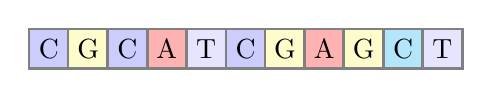
\begin{tikzpicture}
	%\draw[DeepSkyBlue4] decorate{ decorate{ decorate{ (0,0) -- (3,0) }}}; 
	%\pmbchromatogram{SampleScf.scf}
	\DNASequence[Top]{C/blue!20,G/yellow!20,C/blue!20, A/red!30,T/blue!10,C/blue!20, G/yellow!20,A/red!30, G/yellow!20,C/cyan!30,T/blue!10}; 
	
	
	
	%        {C/blue!20, G/blue!20}
	%       {A/cyan!30, G/cyan!30, C/cyan!30};
	
	\end{tikzpicture}
	\\  
	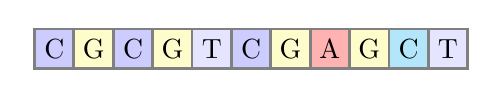
\begin{tikzpicture}
	\hspace*{2pt}\DNASequence[Bottom]{C/blue!20,G/yellow!20,C/blue!20,G/yellow!20,T/blue!10,C/blue!20, G/yellow!20,A/red!30, G/yellow!20,C/cyan!30,T/blue!10}; 
	\end{tikzpicture}
	\\}
\author{Saket Choudhary, Leyla Garcia, Andrew Nightingale}
\institute{University of Southern California, EMBI-EBI}

\begin{document}

\maketitle



\section{Introduction}
\begin{frame}[fragile]
  \frametitle{Sections}
  Sections group slides of the same topic

 
\end{frame}



\begin{frame}[fragile]
  \frametitle{Bioinformatics is broken not broke!}
     

\end{frame}


\begin{frame}{Animation}
  \begin{itemize}[<+- | alert@+>]
    \item \alert<4>{This is\only<4>{ really} important}
    \item Now this
    \item And now this
  \end{itemize}
\end{frame}

\begin{frame}{Figures}
  \begin{figure}
    \newcounter{density}
    \setcounter{density}{20}
    \begin{tikzpicture}
      \def\couleur{mLightBrown}
      \path[coordinate] (0,0)  coordinate(A)
                  ++( 90:5cm) coordinate(B)
                  ++(0:5cm) coordinate(C)
                  ++(-90:5cm) coordinate(D);
      \draw[fill=\couleur!\thedensity] (A) -- (B) -- (C) --(D) -- cycle;
      \foreach \x in {1,...,40}{%
          \pgfmathsetcounter{density}{\thedensity+20}
          \setcounter{density}{\thedensity}
          \path[coordinate] coordinate(X) at (A){};
          \path[coordinate] (A) -- (B) coordinate[pos=.10](A)
                              -- (C) coordinate[pos=.10](B)
                              -- (D) coordinate[pos=.10](C)
                              -- (X) coordinate[pos=.10](D);
          \draw[fill=\couleur!\thedensity] (A)--(B)--(C)-- (D) -- cycle;
      }
    \end{tikzpicture}
    \caption{Rotated square from
    \href{http://www.texample.net/tikz/examples/rotated-polygons/}{texample.net}.}
  \end{figure}
\end{frame}
\begin{frame}{Tables}
  \begin{table}
    \caption{Largest cities in the world (source: Wikipedia)}
    \begin{tabular}{lr}
      \toprule
      City & Population\\
      \midrule
      Mexico City & 20,116,842\\
      Shanghai & 19,210,000\\
      Peking & 15,796,450\\
      Istanbul & 14,160,467\\
      \bottomrule
    \end{tabular}
  \end{table}
\end{frame}
\begin{frame}{Blocks}

  \begin{block}{This is a block title}
    This is soothing.
  \end{block}

\end{frame}
\begin{frame}{Math}
  \begin{equation*}
    e = \lim_{n\to \infty} \left(1 + \frac{1}{n}\right)^n
  \end{equation*}
\end{frame}
\begin{frame}{Line plots}
  \begin{figure}
    \begin{tikzpicture}
      \begin{axis}[
        mlineplot,
        width=0.9\textwidth,
        height=6cm,
      ]

        \addplot {sin(deg(x))};
        \addplot+[samples=100] {sin(deg(2*x))};

      \end{axis}
    \end{tikzpicture}
  \end{figure}
\end{frame}
\begin{frame}{Bar charts}
  \begin{figure}
    \begin{tikzpicture}
      \begin{axis}[
        mbarplot,
        xlabel={Foo},
        ylabel={Bar},
        width=0.9\textwidth,
        height=6cm,
      ]

      \addplot plot coordinates {(1, 20) (2, 25) (3, 22.4) (4, 12.4)};
      \addplot plot coordinates {(1, 18) (2, 24) (3, 23.5) (4, 13.2)};
      \addplot plot coordinates {(1, 10) (2, 19) (3, 25) (4, 15.2)};

      \legend{lorem, ipsum, dolor}

      \end{axis}
    \end{tikzpicture}
  \end{figure}
\end{frame}
\begin{frame}{Quotes}
  \begin{quote}
    Veni, Vidi, Vici
  \end{quote}
\end{frame}


\section{Conclusion}

\begin{frame}{Summary}

  Get the source of this theme and the demo presentation from

  \begin{center}\url{github.com/matze/mtheme}\end{center}

  The theme \emph{itself} is licensed under a
  \href{http://creativecommons.org/licenses/by-sa/4.0/}{Creative Commons
  Attribution-ShareAlike 4.0 International License}.

  \begin{center}\ccbysa\end{center}

\end{frame}

\plain{Questions?}

\end{document}
